\documentclass[12pt]{report}
\usepackage[a3paper]{geometry}
\usepackage{multirow}
\usepackage{graphicx}
\usepackage{color}
\usepackage{hyperref}
\usepackage{enumerate}
\usepackage{amsthm}
\usepackage{amssymb}
\usepackage{listings}
\usepackage{pdflscape}
\usepackage{color, colortbl}
\usepackage[table]{xcolor}
\usepackage{longtable}
\usepackage{tabularx}
\geometry{total={297mm, 420mm}, left=20mm, right=22mm, top=25mm, bottom=25mm}

\hypersetup{
    pdffitwindow=true,
    pdfstartview={FitH},
    colorlinks=true,
    linkcolor=blue,
    citecolor=red,
    urlcolor=blue
}

\lstset{
    basicstyle=\footnotesize,
    numbers=left,
    numberstyle=\footnotesize,
    stepnumber=1,
    numbersep=5pt,
    frame=single,
    breaklines=true,
    title=\lstname
}

\sloppy
\newtheorem{definition}{Definition}

\begin{document}
\author{Krzysztof Jusiak}
\title{C++ FSM frameworks comparison}
\frenchspacing
\maketitle

\begin{abstract}
Document presents comparison between C++ FSM frameworks:
\begin{itemize}
\item Boost Meta State Machine (msm)
\item Boost State Chart (statechart)
\item Quick Finite State Machine (QFsm)
\end{itemize}
\end{abstract}

\clearpage
\tableofcontents
\clearpage
\subsection{Results from "server" [df6407d], generated Sun Sep 25 23:45:00 CEST 2011}
\begin{verbatim}

Test aspects:

    compilation:
        compilation time measured by 'time' call
        only 'real' time is taken into account
        result is in seconds

    size:
        size of the binary measured by 'ls -k' call
        result is in kilobytes

    strip-size:
        size of the binary measured by 'ls -k' call after 'strip' call
        result is in kilobytes

    execution:
        execution time measured by 'time' call
        only 'real' time is taken into account
        result is in seconds

    valgrind:
        test is executed with valgrind call
        result is as A/D (S), where
        A - allocations
        D - deallocations
        S - global allocated size in bytes

    test name:
        test_NAME[_NUMBER], where NAME is test case name and NUMBER is count of event calls during the test
\end{verbatim}
\begin{center}
\line(1,0){750}
\end{center}
\begin{verbatim}

Environment statistics:

    generated: Sun Sep 25 23:45:00 CEST 2011
    code revision: df6407d
    hostname: "server"
    operating system:  GNU/Linux
    processor: x86_64
    free memory: 1748Mb
    load average: 1.30 1.39 1.28 1/626 16681

\end{verbatim}
\begin{center}
\line(1,0){750}
\end{center}
\begin{verbatim}

All tests summary:

    real: 593.18s (9:53.18)
    user: 579.98s
    sys: 10.70s
    cpu: 99%
    average memory usage: 0K
    maximum resident set size: 2866352K
    number of times the process was swapped out of main memory: 0
    number of file system input: 120
    number of file system outputs: 466288
\end{verbatim}
\begin{center}
\line(1,0){750}
\end{center}
\begin{verbatim}
Results are presented by using table and two types of charts:

    table: contains results for each tested aspect and framework
    first type of chart: presents relative (0-100%) differents between individual framework and aspect
    second type of chart: presents each aspect individually using exact values returned during the test
\end{verbatim}
\begin{center}
\line(1,0){750}
\end{center}
\begin{landscape}
\begin{table}
\caption{"server" [54c084f], g++44 -m32 -O2 -DNDEBUG/test transitions 1000000}
\centering
\begin{longtable}{| c | c |c |c |c |c |c |c |}
\hline
& CFsmBase& StateChart& MSM.favor\_runtime\_speed& MSM.favor\_compile\_time& QFsm.FavorExecutionSpeed& QFsm.FavorCompilationTime& QFsm.FavorDebugSize\\
\hline
compilation & 0.96s & 1.12s & 2.22s & 2.24s & 0.54s & 0.45s & 0.70s\\
\hline
size & 41K & 31K & 29K & 31K & 11K & 8K & 18K\\
\hline
strip-size & 29K & 18K & 16K & 16K & 6K & 5K & 11K\\
\hline
execution & 0.04s & 0.11s & 0.00s & 0.02s & 0.00s & 0.00s & 0.01s\\
\hline
valgrind & 9/9 (138b) & 1,000,004/1,000,004 (24,000,064b) & 4/4 (561b) & 10/10 (2,673b) & 2/2 (17b) & 2/2 (17b) & 16/16 (241b)\\
\hline
\multicolumn{8}{|c|}{\includegraphics[scale=0.8]{images/"results/server"/"g++44 -m32 -O2 -DNDEBUG"/test_transitions_1000000_all.png}}\\
\hline
\end{longtable}
\end{table}
\end{landscape}
\newpage
\begin{table}
\centering
\begin{longtable}{| c | c |}
\hline
\includegraphics[scale=0.8]{images/"results/server"/"g++44 -m32 -O2 -DNDEBUG"/test_transitions_1000000_compilation.png}& \includegraphics[scale=0.8]{images/"results/server"/"g++44 -m32 -O2 -DNDEBUG"/test_transitions_1000000_size.png}\\
\hline
\includegraphics[scale=0.8]{images/"results/server"/"g++44 -m32 -O2 -DNDEBUG"/test_transitions_1000000_strip-size.png}& \includegraphics[scale=0.8]{images/"results/server"/"g++44 -m32 -O2 -DNDEBUG"/test_transitions_1000000_execution.png}\\
\hline
\includegraphics[scale=0.8]{images/"results/server"/"g++44 -m32 -O2 -DNDEBUG"/test_transitions_1000000_valgrind.png}& \\ \hline
\end{longtable}
\end{table}
\begin{landscape}
\begin{table}
\caption{"server" [54c084f], g++44 -m32 -O2 -DNDEBUG/test complex 1000000}
\centering
\begin{longtable}{| c | c |c |c |c |c |c |c |}
\hline
& CFsmBase& StateChart& MSM.favor\_runtime\_speed& MSM.favor\_compile\_time& QFsm.FavorExecutionSpeed& QFsm.FavorCompilationTime& QFsm.FavorDebugSize\\
\hline
compilation & 1.13s & 1.90s & 10.30s & 8.32s & 21.79s & 1.52s & 2.35s\\
\hline
size & 51K & 63K & 225K & 253K & 89K & 21K & 70K\\
\hline
strip-size & 35K & 31K & 33K & 47K & 10K & 8K & 37K\\
\hline
execution & 0.18s & 0.12s & 0.01s & 0.02s & 0.00s & 0.01s & 0.05s\\
\hline
valgrind & 26/26 (449b) & 1,000,014/1,000,014 (24,000,204b) & 14/14 (646b) & 122/122 (38,662b) & 12/12 (102b) & 12/12 (102b) & 235/235 (4,718b)\\
\hline
\multicolumn{8}{|c|}{\includegraphics[scale=0.8]{images/"results/server"/"g++44 -m32 -O2 -DNDEBUG"/test_complex_1000000_all.png}}\\
\hline
\end{longtable}
\end{table}
\end{landscape}
\newpage
\begin{table}
\centering
\begin{longtable}{| c | c |}
\hline
\includegraphics[scale=0.8]{images/"results/server"/"g++44 -m32 -O2 -DNDEBUG"/test_complex_1000000_compilation.png}& \includegraphics[scale=0.8]{images/"results/server"/"g++44 -m32 -O2 -DNDEBUG"/test_complex_1000000_size.png}\\
\hline
\includegraphics[scale=0.8]{images/"results/server"/"g++44 -m32 -O2 -DNDEBUG"/test_complex_1000000_strip-size.png}& \includegraphics[scale=0.8]{images/"results/server"/"g++44 -m32 -O2 -DNDEBUG"/test_complex_1000000_execution.png}\\
\hline
\includegraphics[scale=0.8]{images/"results/server"/"g++44 -m32 -O2 -DNDEBUG"/test_complex_1000000_valgrind.png}& \\ \hline
\end{longtable}
\end{table}
\begin{landscape}
\begin{table}
\caption{"server" [54c084f], g++44 -m32 -Os -DNDEBUG/test transitions 1000000}
\centering
\begin{longtable}{| c | c |c |c |c |c |c |c |}
\hline
& CFsmBase& StateChart& MSM.favor\_runtime\_speed& MSM.favor\_compile\_time& QFsm.FavorExecutionSpeed& QFsm.FavorCompilationTime& QFsm.FavorDebugSize\\
\hline
compilation & 0.90s & 0.91s & 2.18s & 2.21s & 0.55s & 0.45s & 0.65s\\
\hline
size & 40K & 28K & 26K & 30K & 11K & 8K & 16K\\
\hline
strip-size & 28K & 13K & 12K & 14K & 5K & 5K & 9K\\
\hline
execution & 0.05s & 0.16s & 0.01s & 0.02s & 0.00s & 0.00s & 0.01s\\
\hline
valgrind & 9/9 (138b) & 1,000,004/1,000,004 (24,000,064b) & 4/4 (561b) & 10/10 (2,673b) & 2/2 (17b) & 2/2 (17b) & 16/16 (241b)\\
\hline
\multicolumn{8}{|c|}{\includegraphics[scale=0.8]{images/"results/server"/"g++44 -m32 -Os -DNDEBUG"/test_transitions_1000000_all.png}}\\
\hline
\end{longtable}
\end{table}
\end{landscape}
\newpage
\begin{table}
\centering
\begin{longtable}{| c | c |}
\hline
\includegraphics[scale=0.8]{images/"results/server"/"g++44 -m32 -Os -DNDEBUG"/test_transitions_1000000_compilation.png}& \includegraphics[scale=0.8]{images/"results/server"/"g++44 -m32 -Os -DNDEBUG"/test_transitions_1000000_size.png}\\
\hline
\includegraphics[scale=0.8]{images/"results/server"/"g++44 -m32 -Os -DNDEBUG"/test_transitions_1000000_strip-size.png}& \includegraphics[scale=0.8]{images/"results/server"/"g++44 -m32 -Os -DNDEBUG"/test_transitions_1000000_execution.png}\\
\hline
\includegraphics[scale=0.8]{images/"results/server"/"g++44 -m32 -Os -DNDEBUG"/test_transitions_1000000_valgrind.png}& \\ \hline
\end{longtable}
\end{table}
\begin{landscape}
\begin{table}
\caption{"server" [54c084f], g++44 -m32 -Os -DNDEBUG/test complex 1000000}
\centering
\begin{longtable}{| c | c |c |c |c |c |c |c |}
\hline
& CFsmBase& StateChart& MSM.favor\_runtime\_speed& MSM.favor\_compile\_time& QFsm.FavorExecutionSpeed& QFsm.FavorCompilationTime& QFsm.FavorDebugSize\\
\hline
compilation & 0.96s & 1.66s & 9.70s & 7.49s & 21.42s & 1.58s & 2.19s\\
\hline
size & 47K & 58K & 214K & 243K & 87K & 20K & 62K\\
\hline
strip-size & 31K & 25K & 21K & 34K & 8K & 7K & 32K\\
\hline
execution & 0.17s & 0.17s & 0.02s & 0.03s & 0.01s & 0.02s & 0.09s\\
\hline
valgrind & 26/26 (449b) & 1,000,014/1,000,014 (24,000,204b) & 14/14 (646b) & 122/122 (38,662b) & 12/12 (102b) & 12/12 (102b) & 235/235 (4,718b)\\
\hline
\multicolumn{8}{|c|}{\includegraphics[scale=0.8]{images/"results/server"/"g++44 -m32 -Os -DNDEBUG"/test_complex_1000000_all.png}}\\
\hline
\end{longtable}
\end{table}
\end{landscape}
\newpage
\begin{table}
\centering
\begin{longtable}{| c | c |}
\hline
\includegraphics[scale=0.8]{images/"results/server"/"g++44 -m32 -Os -DNDEBUG"/test_complex_1000000_compilation.png}& \includegraphics[scale=0.8]{images/"results/server"/"g++44 -m32 -Os -DNDEBUG"/test_complex_1000000_size.png}\\
\hline
\includegraphics[scale=0.8]{images/"results/server"/"g++44 -m32 -Os -DNDEBUG"/test_complex_1000000_strip-size.png}& \includegraphics[scale=0.8]{images/"results/server"/"g++44 -m32 -Os -DNDEBUG"/test_complex_1000000_execution.png}\\
\hline
\includegraphics[scale=0.8]{images/"results/server"/"g++44 -m32 -Os -DNDEBUG"/test_complex_1000000_valgrind.png}& \\ \hline
\end{longtable}
\end{table}
\begin{landscape}
\begin{table}
\caption{"server" [54c084f], g++44 -m32 -g/test transitions 1000000}
\centering
\begin{longtable}{| c | c |c |c |c |c |c |c |}
\hline
& CFsmBase& StateChart& MSM.favor\_runtime\_speed& MSM.favor\_compile\_time& QFsm.FavorExecutionSpeed& QFsm.FavorCompilationTime& QFsm.FavorDebugSize\\
\hline
compilation & 0.90s & 1.07s & 2.43s & 2.48s & 0.77s & 0.67s & 0.72s\\
\hline
size & 167K & 445K & 670K & 762K & 188K & 117K & 191K\\
\hline
strip-size & 23K & 48K & 34K & 40K & 9K & 8K & 18K\\
\hline
execution & 0.11s & 1.08s & 0.61s & 0.71s & 0.08s & 0.12s & 0.26s\\
\hline
valgrind & 9/9 (138b) & 1,000,004/1,000,004 (24,000,064b) & 4/4 (561b) & 10/10 (2,673b) & 2/2 (17b) & 2/2 (17b) & 16/16 (241b)\\
\hline
\multicolumn{8}{|c|}{\includegraphics[scale=0.8]{images/"results/server"/"g++44 -m32 -g"/test_transitions_1000000_all.png}}\\
\hline
\end{longtable}
\end{table}
\end{landscape}
\newpage
\begin{table}
\centering
\begin{longtable}{| c | c |}
\hline
\includegraphics[scale=0.8]{images/"results/server"/"g++44 -m32 -g"/test_transitions_1000000_compilation.png}& \includegraphics[scale=0.8]{images/"results/server"/"g++44 -m32 -g"/test_transitions_1000000_size.png}\\
\hline
\includegraphics[scale=0.8]{images/"results/server"/"g++44 -m32 -g"/test_transitions_1000000_strip-size.png}& \includegraphics[scale=0.8]{images/"results/server"/"g++44 -m32 -g"/test_transitions_1000000_execution.png}\\
\hline
\includegraphics[scale=0.8]{images/"results/server"/"g++44 -m32 -g"/test_transitions_1000000_valgrind.png}& \\ \hline
\end{longtable}
\end{table}
\begin{landscape}
\begin{table}
\caption{"server" [54c084f], g++44 -m32 -g/test complex 1000000}
\centering
\begin{longtable}{| c | c |c |c |c |c |c |c |}
\hline
& CFsmBase& StateChart& MSM.favor\_runtime\_speed& MSM.favor\_compile\_time& QFsm.FavorExecutionSpeed& QFsm.FavorCompilationTime& QFsm.FavorDebugSize\\
\hline
compilation & 0.98s & 2.06s & 16.37s & 13.95s & 32.26s & 2.79s & 2.22s\\
\hline
size & 208K & 1323K & 23490K & 29254K & 13685K & 7720K & 843K\\
\hline
strip-size & 31K & 127K & 131K & 171K & 31K & 57K & 63K\\
\hline
execution & 0.21s & 1.49s & 0.80s & 0.97s & 0.10s & 0.44s & 1.01s\\
\hline
valgrind & 26/26 (449b) & 1,000,014/1,000,014 (24,000,204b) & 14/14 (646b) & 122/122 (38,662b) & 12/12 (102b) & 12/12 (102b) & 235/235 (4,718b)\\
\hline
\multicolumn{8}{|c|}{\includegraphics[scale=0.8]{images/"results/server"/"g++44 -m32 -g"/test_complex_1000000_all.png}}\\
\hline
\end{longtable}
\end{table}
\end{landscape}
\newpage
\begin{table}
\centering
\begin{longtable}{| c | c |}
\hline
\includegraphics[scale=0.8]{images/"results/server"/"g++44 -m32 -g"/test_complex_1000000_compilation.png}& \includegraphics[scale=0.8]{images/"results/server"/"g++44 -m32 -g"/test_complex_1000000_size.png}\\
\hline
\includegraphics[scale=0.8]{images/"results/server"/"g++44 -m32 -g"/test_complex_1000000_strip-size.png}& \includegraphics[scale=0.8]{images/"results/server"/"g++44 -m32 -g"/test_complex_1000000_execution.png}\\
\hline
\includegraphics[scale=0.8]{images/"results/server"/"g++44 -m32 -g"/test_complex_1000000_valgrind.png}& \\ \hline
\end{longtable}
\end{table}


\clearpage
\listoffigures
\listoftables

\end{document}

